%!TEX root = ../../../../../memoria.tex
\section{Formularios}

Los formularios son parte relevante de la aplicación. Por lo tanto se puse especial énfasis en 

\subsection{Pocos campos en los formularios}
Cada uno de los formularios que existen en la aplicación fueron creados con este principio. Los seres humanos son intrínsecamente resistentes a labores de tareas intensivas y el mismo principio se aplica para llenar completamente un formulario. Por cada campo agregado al formulario, se corre el riesgo de perder un cliente\cite{online_goodgui_org}.
%TODO : Agregar referencia a figura de creación de usuario
Un caso claro de esto, corresponde a la interfaz de creación de un usuario ( \refFigura{figure:account:create_account:form}), la cual fue diseñada solo con dos campos.


\subsection{Errores}
Los errores ocurriran sin importar las medidas que se tomen. Lo importante es evitar al máximo que estos sucedan. Y cuando esto pase, guiar adecuadamente al usuario para que pueda resolver los problemas sin mayores inconvenientes. Para estos casos se debe proceder de la manera siguiente:
\begin{itemize}
	\item Comunicar claramente que es aquello que esta sucediendo.
	\item Describir como el usuario puede resolverlo.
	\item Mantener tanto \inputBrowserINT del usuario como sea posible \cite{online_google_ui_pattern_error}.
\end{itemize} 


\begin{figure}[H]
	\centering
	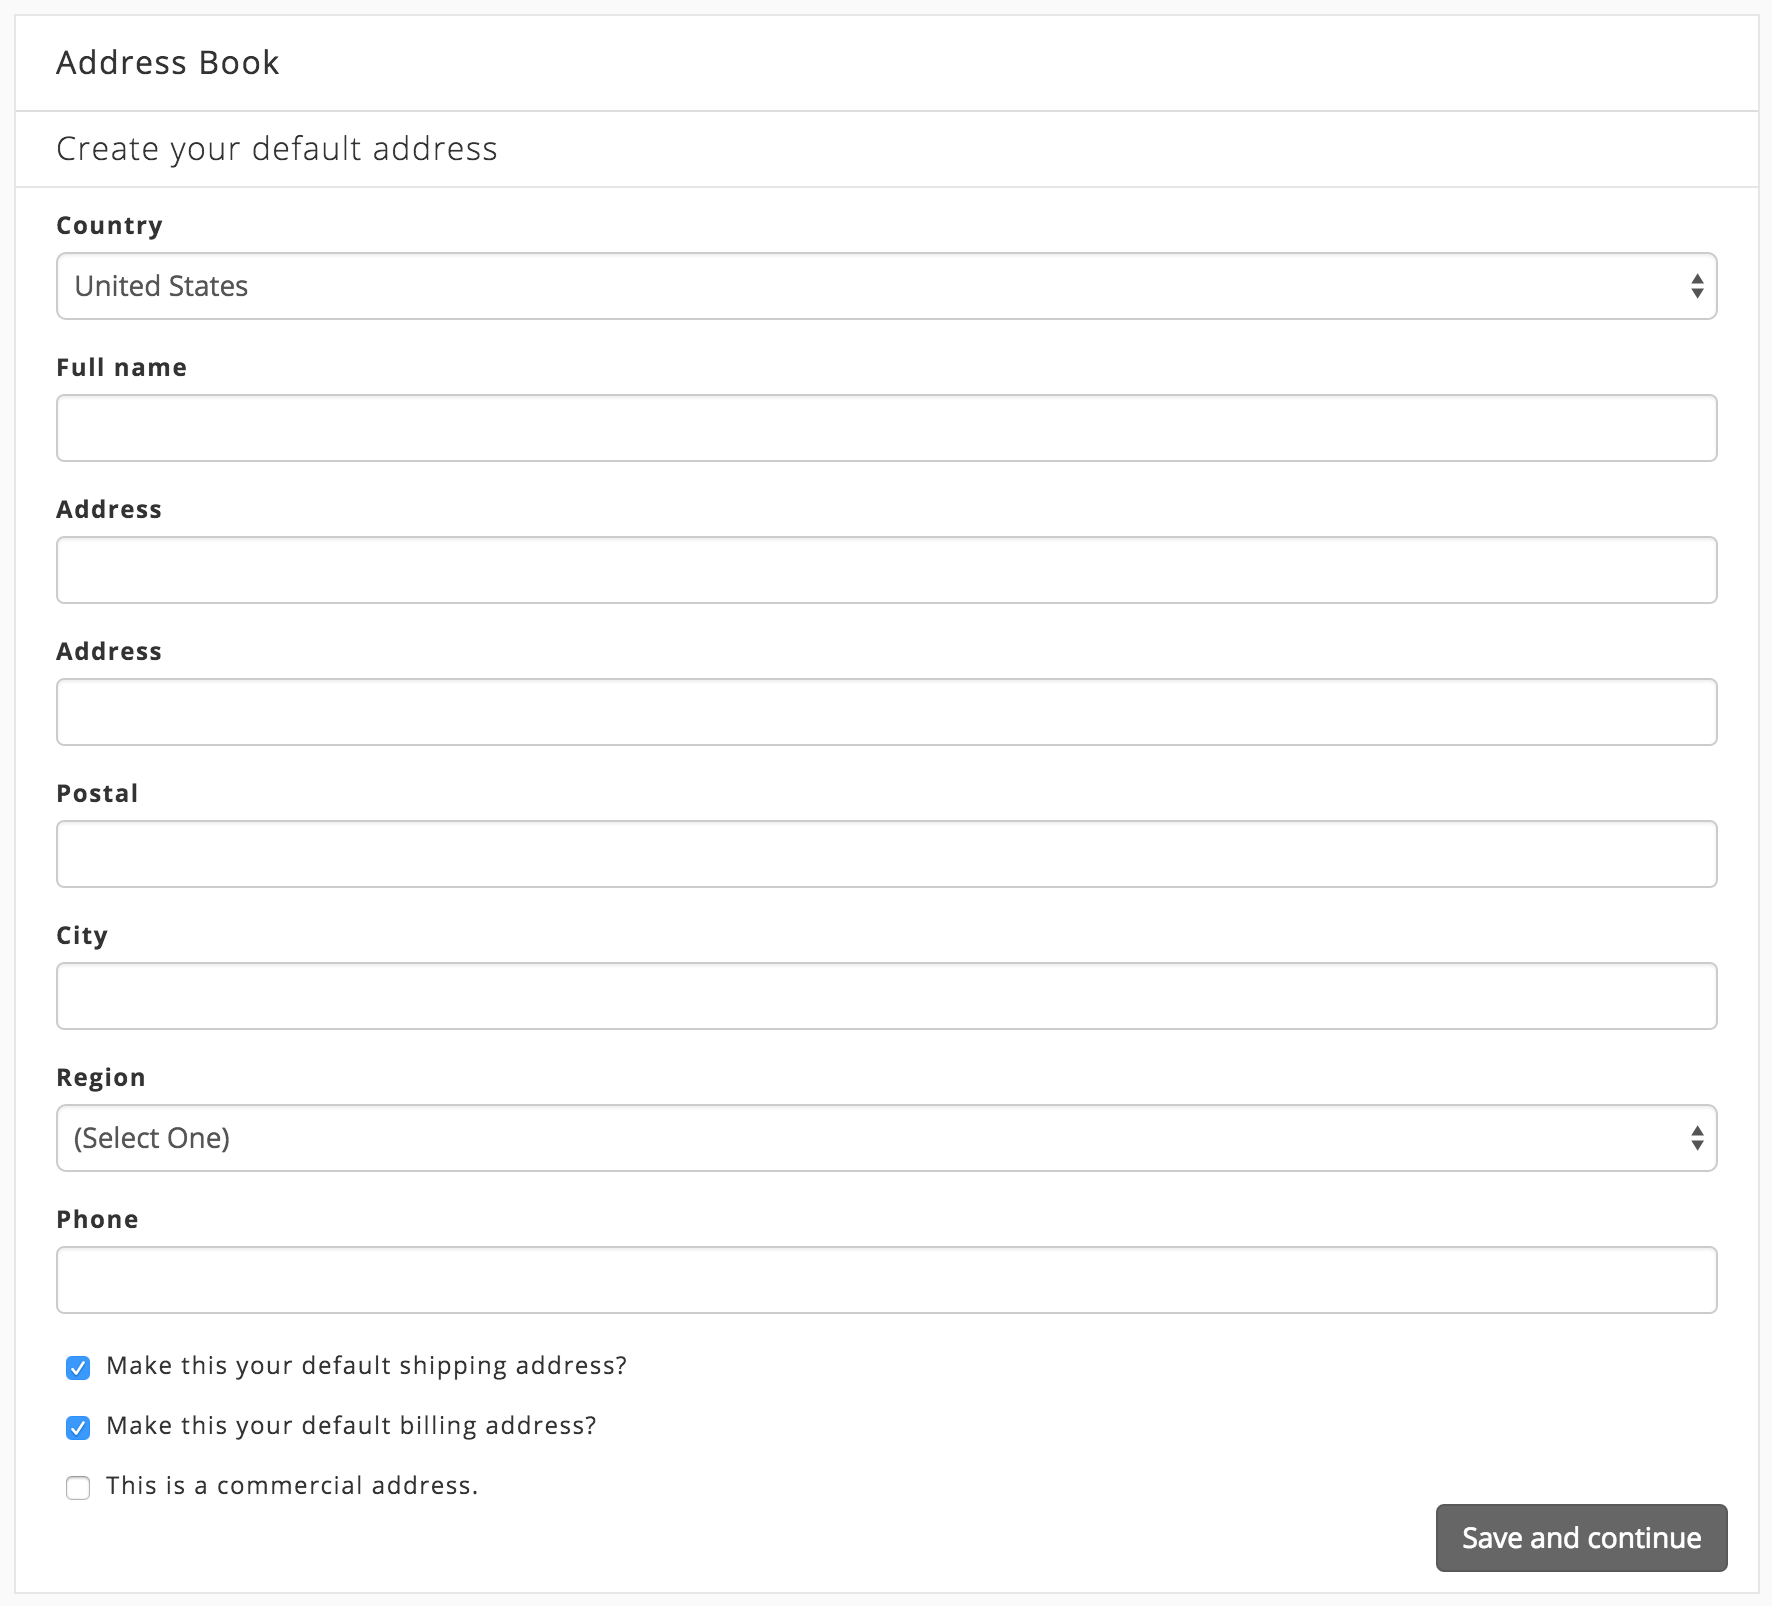
\includegraphics[width=0.5\textwidth]{figuras/formularios/form_address_book.png}

	\caption{Formulario de creación de una nueva dirección de envio.}
	\label{figure:form:form_address_book}
\end{figure}













